\setcounter{page}{1}
\artigofalse
\chapter{General introduction}
\label{chap:introduction}

\section{Background and motivation}

\subsection{Demand for soil information}

Soil science is experiencing a period of renaissance that started in the last 
decade \cite{HarteminkEtAl2008}. It is a result of a new global demand for soil 
information needed to solve what has been defined as the five major problems of
our time: food security, climate change, environmental degradation, water 
scarcity and threats to the biodiversity \cite{SanchezEtAl2009}. The Food and 
Agriculture Organization (\href{http://www.fao.org/index_en.htm}{FAO}) of the 
United Nations (\href{http://www.un.org/en/}{UN}), through the Global Soil 
Partnership (\href{http://www.fao.org/globalsoilpartnership/en/}{GSP}) project, 
is the main global demander of up-to-date soil information. The objective of 
FAO is to support and ensure the implementation of joint efforts that lead to 
the adoption of sustainable development goals for the soils \cite{FAO2012}. 
Digital soil mapping (DSM), \textit{the} \textit{creation and population of 
spatial soil information systems through the use of field and laboratory 
observational methods, coupled with spatial and non-spatial soil inference 
systems} \cite{LagacherieEtAl2007a}, a branch of pedometrics, a new emerging 
discipline of soil science that corresponds to the \textit{application of 
mathematical and statistical methods for the study of the distribution and 
genesis of soils} \cite{Heuvelink2003}, is the best alternative to meet this 
new demand for soil information. This is because DSM addresses the main 
problems of the classical approach of soil mapping \cite{Kempen2011}. First, 
DSM is data-centered (\textit{environmental-centered}) and gives emphasis on 
producing soil information according to the needs of soil information users 
(\textit{user-driven}). Second, DSM relies on using well documented statistical
models (\textit{reproducible research}) that allow treating the soil as a 
continuum (models of spatial variation). And third, DSM products can be made 
available at a lower cost in soil information systems with quantified 
uncertainty.

Several initiatives have been undertaken around the world in the last years to 
ensure the development and implementation of DSM. The main examples are the 
GlobalSoilMap.net consortium and ISRIC's Global Soil Information Facilities
(\href{http://www.isric.org/projects/global-soil-information-facilities-gsif}{GSIF}).
In Brazil, soil scientists created the Brazilian Network for Research in DSM 
(RedeMDS) with the main objective of generating synergy among Brazilian soil 
scientists to advance the research in DSM in Brazil \cite{RedeMDS2013}. Also, 
the two first job positions for assistant professors in Pedometrics and DSM in 
Brazilian universities were created in 2011 and 2013 \cite{UFRRJ2011,UFSM2012}. 
Unfortunately these local initiatives are not supported by any official 
government demand for up-to-date soil information in Brazil 
\cite{SamuelRosa2012}. Several economic, politic and cultural reasons have been 
pointed out to explain the lack of interest on soil information in Brazil since 
the 1980s \cite{Dalmolin1999, Ker1999, KerEtAl2003, Ramos2003, Espindola2008}, 
but their resolution is out of the scope of this thesis. Alike many other local
initiatives, the present thesis complies with the priorities defined by the 75 
soil scientists from 17 countries that came together in Rio de Janeiro on July 
2006 during the 2nd Global Workshop on Digital Soil Mapping, for whom developing
and implementing DSM depends on training students and experienced soil 
scientists, standardizing methods and measures, and building international 
collaboration \cite{Boettinger2004}.

\subsection{Modern soil mapping} %%%%%%%%%%%%%%%%%%%%%%%%%%%%%%%%%%%%%%%%%%%%%%%%%%%%%%%%%%%%%%%%%%%

In general terms, the DSM framework can be described as a series of seven steps 
as follows:

\begin{description}
  \item [{Step~0}] Identify a reality or problem entity: geographic region where
  pedometric techniques will be used to model the soil property(ies) distribution
  in the geographic and attribute spaces in a given time period;

  \item [{Step~1}] Develop a conceptual model of pedogenesis: verbal 
  representation of the reality or problem entity including the explicit 
  description of soil forming factors and processes that drive soil 
  characteristics and its spatial distribution pattern. This step relies on 
  gathering all environmental information available and applying concepts 
  (expert knowledge) of soil-landscape system, catenary soil development or 
  other theoretical model of explanation of soil spatial variation;

  \item [{Step~2}] Develop a mathematical representation: translate the verbal 
  representation of the reality or problem entity into a set of possible 
  mathematical representations. In this step we use the conceptual model of 
  pedogenesis to define the sample design and the number of soil observations 
  needed to calibrate the DSM model, collect predictor variables from available 
  environmental ancillary data (environmental covariates), specify model 
  structure (linear or non-linear) and define the techniques to be used in the 
  remainder of the DSM modelling activity (tests of independence, normality and 
  homoscedasticity, multicollinearity assessment, variable selection method, 
  goodness-of-fit measures, etc). Several of this tasks can be (and usually are)
  carried out with the aid of a data processing environment such as a computer;

  \item [{Step~3}] Develop a computer representation: translate the set of 
  mathematical representations of the reality or problem entity into a computer 
  representation, that is, a computer code or computer script. The computer 
  code is used to establish the communication between the DSM modeller (a human 
  being) and the data processing environment (a computer) where mathematical 
  representations and DSM model assessment tools are implemented. Developing a 
  computer code that describes all processing steps is at the core of the 
  concept of \textit{reproducible research} in DSM;

  \item [{Step~4}] Data analysis: run the computer code and evaluate the 
  outcomes. This includes the univariate analysis and selection of candidate 
  predictor variables, followed by its multivariate analysis, and evaluation of
  the adequacy of multivariate model(s), namely check model assumptions, look 
  for interactions between predictor variables, evaluate goodness-of-fit 
  measures and visually assess preliminary soil maps. Best performing DSM 
  model(s) are evaluated regarding their tenability (pedological evaluation) 
  and how well they represent the range of possible mathematical models. 
  Failure in this last assessment means that DSM model(s) have to be adjusted 
  and data analysis rerun, or can simply be discarded;

  \item [{Step~5}] Make predictions: application of best performing DSM model(s)
  to predict soil property values and confidence interval at unvisited locations;

  \item [{Step~6}] Statistical validation: validate the set of DSM models using
  existing independent field data and select the best performing model using a 
  statistical criterion. Best performing DSM model is assumed to be the best 
  mathematical representation of the reality or problem entity under 
  consideration. If previous steps have already allowed selecting a single best 
  performing DSM model, statistical validation is used only to assess model 
  accuracy;
  
  \item [{Step~7}] Reformulate the conceptual model of pedogenesis: selected 
  DSM model and prediction and uncertainty maps can provide new insights about 
  the reality or problem entity, and thus allow reformulating or improving the 
  verbal representation of the conceptual model of pedogenesis;
  
  \item [{Step~8}] Populate spatial soil information systems: point soil 
  observations, prediction and uncertainty maps, and metadata are used to 
  populate a spatial soil information system and made available for inspection 
  through different visualization techniques.
\end{description}

\subsection{Sources of uncertainty} %%%%%%%%%%%%%%%%%%%%%%%%%%%%%%%%%%%%%%%%%%%%%%%%%%%%%%%%%%%%%%%%

Soil-mapping models, like any other model, are nothing more than a gross simplification of reality.
This means that soil-mapping models are unable to explain the spatio-temporal soil variation in 
its entirety, but only a small part of it \citep{Heuvelink1998a}. When we use a soil-mapping model
to produce continuous representations of soil properties across space and/or time, i.e. soil
maps, these continuous representations will inexorably deviate from the ``truth''. What the soil map
presents is our most likely expectation about the soil properties -- not our \textit{certainty} about
about them. The deviation from the ``truth'' is what we call \textit{error}. Many examples from the 
soil-mapping literature show that, irrespective of the soil property, soil-mapping models have a 
quite variable predictive performance, usually explaining between 15\% (or less) and (rarely more 
than) 75\% of the spatio-temporal soil variation \citep{MooreEtAl1993, OdehEtAl1994, GesslerEtAl1995, 
McKenzieEtAl1999, GobinEtAl2001, SumflethEtAl2008, SunEtAl2012, ViscarraRosselEtAl2013, 
NussbaumEtAl2014, HenglEtAl2015, GaschEtAl2015, HeungEtAl2016}.

The main reason for a soil map to be in error is that the background knowledge and data used to 
construct the soil-mapping model is very limited -- we have to try our best with the available 
resources. Unless we observe the soil everywhere, which would destroy the soil and render the 
observations useless, no matter how large the volume of data is, or how comprehensive our background
knowledge is, it will never be possible to construct a model that explains the entire complexity of 
the soil \citep{Tukey1997}. This means that our knowledge about the soil, and the world as a whole, 
will always be only partial \citep{Box1993}. Because we cannot eliminate the uncertainty of a soil 
map, they can always be considered as wrong, the difference being that some might be useful 
\citep{Box1976}.

Soil modellers/mappers aim at producing the most accurate representations of the soil given the 
available resources. Thus, a reasonable research program is the identification of the causes for 
soil maps being more or less uncertain. For instance, the error that results from making 
extrapolations and interpolations to predict the soil properties at unvisited locations is an 
important source of uncertainty \citep{HeuvelinkEtAl1999, RefsgaardEtAl2006}. Because modern soil 
mapping is \textit{data-centred}, these errors are larger the farther we are from the existing 
observations. Thus, the most efficient way of reducing these errors is to increase the number of 
observations and improve the spatial coverage of the mapping region (BrusEtAl2007a). However, most 
soil-mapping projects must rely on using only soil data produced many years ago \citep{KempenEtAl2009, 
HenglEtAl2014, PoggioEtAl2014, NussbaumEtAl2014, MulderEtAl2016}, when most sampling locations were 
defined based on the tacit knowledge of soil surveyors -- that usually place more samples in complex 
and less known areas \citep{Rossiter2000} -- or other poorly documented criteria.

On the contrary, if the budget of the soil-mapping project includes (additional) sampling, soil 
modellers/mappers have to decide upon the number and spatial configuration of the sample 
\citep{deGruijterEtAl2006, WebsterEtAl2013}. Unfortunately this is not an easy task, except if the 
goal is on mapping/modelling very few soil properties that can be rapidly measured using field 
sensors, and for which a model of spatial (co)variation can be assumed known \citep{MarchantEtAl2006}.
In most cases, several difficult-to-measure soil properties have to be modelled/mapped, many of 
which have a poorly known structure of spatial (co)variation. The chosen spatial sample configuration
has to be appropriate for estimating the spatial trend \citep{HenglEtAl2003a, MinasnyEtAl2006b} and 
the variogram model \citep{WarrickEtAl1987, WebsterEtAl1992, Lark2002}, making spatial predictions 
\citep{YfantisEtAl1987, WalvoortEtAl2010} and, (cross)validating the model/map \citep{BrusEtAl2011}, 
four often conflicting objectives. Besides, one must be careful not to decide upon collecting an 
insufficient or an exaggerated number of samples. Sub-sampling can result in soil-mapping models 
with little utility, while over-sampling can produce modelling benefits that do not outweigh the
sampling costs \citep{vanGroenigenEtAl1999}.

Soil data may not only poorly cover the geographic and/or feature spaces \citep{HenglEtAl2003a}, but
also have significant laboratory and positional errors \citep{NelsonEtAl2011}. Besides, some soil 
properties may naturally contain more errors due to their conceptual definition and analytical 
procedures employed. Take particle-size distribution as an example. First, the errors are propagated
to the fraction obtained by difference (silt). Second, pre-treatments, such as organic matter 
oxidation, can change mineral structure \citep{MikuttaEtAl2005a}. And third, ignoring that the 
particle-size distribution is a compositional datum can introduce bias in the predictions 
\citep{LarkEtAl2007}.

Another important source of uncertainty is the covariates used to calibrate the soil-mapping models.
First, because they contain varying levels of error \citep{HeuvelinkEtAl1989}. These errors derive 
from the various methods of data generation, analytical procedures and, inherent characteristics of 
each site. For example, digital elevation models usually present larger errors in areas with steep 
slopes, rough terrains, and great elevations, and with dense forest cover or urbanized 
\citep{Florinsky1998, Toutin2000, FisherEtAl2006}. Interpolation of elevation data using kriging 
can produce spurious artefacts \citep{HenglEtAl2009} compared to hydrologically consistent 
algorithms \citep{Hutchinson1989}. And stereoscopic correlation techniques produce digital elevation
models with poorer quality than interferometric synthetic aperture radar \citep{HirtEtAl2010}.

Deciding upon which covariates to include in the soil-mapping model is another important source of 
uncertainty. This is specially important now days, when the number of available (uncertain) 
covariates increases every week, many of which possibly being statistically redundant. A 
pedologically sound approach for selecting the covariates consists in eliciting the knowledge of a 
few experts \citep{LarkEtAl2007b}, optimally more than five \citep{MeyerEtAl2001}. An expert is 
every soil modeller/mapper with long practical experience and large pedological, mathematical, and 
statistical knowledge \citep{MeyerEtAl2001}. If the mapping region is unknown to the expert, then
a sound \textit{conceptual model of pedogenesis} must be provided. However, the understanding
about the mapping region may be limited to a point that enables building only a very uncertain 
conceptual model of pedogenesis. For example, a unstable landscape that consistently suffers natural
and/or anthropogenic alterations is geomorphologically more complex than a stable one 
\citep{Schumm1979}. As the complexity increases, and the landscape is rejuvenated, establishing 
soil-landscape relationships becomes very difficult \citep{StreckEtAl2008}. Similar uncertainty 
in the conceptual model of pedogenesis can arise in very old, stable geomorphic surfaces that have 
gone through many environmental modifications, but were not affected by Pleistocene glaciations 
\citep{McKenzieEtAl2000a}. These landscapes commonly have polygenetic soils that present properties
reflecting today but ancient vegetation and climate \citep{PainEtAl1995, Ker1998a}.

A most used approach to select the covariates to enter a soil-mapping model is automated selection.
Because automated selection algorithms are available in most software packages \citep{Harrell2001}, 
are relatively easy to use \citep{DraperEtAl1971}, deliver satisfactory results, 
\citep{HenglEtAl2004}, and are needed to automate soil-mapping routines \citep{HenglEtAl2014}. The 
main uncertainty here is on which method to use. Some methods analyse all possible combinations of 
covariates. Others simulate the process of natural selection \citep{AndersenEtAl2010}. 
Cross-validation selects covariates that produce the best predictions on test sets 
\citep{GuyonEtAl2003}. Other methods take into account the order in which the covariates are added 
to (forward selection) or removed from (backward elimination) the model \citep{LarkEtAl2007a}. And 
the stepwise method adds and removes covariates until no further addition or removal results in 
significant changes in the model \citep{Efroymson1962}. Many other methods exist and have been 
already used in soil-mapping projects \citep{PoggioEtAl2013, NussbaumEtAl2014}. Some prefer to use 
dimensionality reduction techniques to reduce the number of covariates \citep{Massy1965} before 
running the covariate selection algorithm \citep{tenCatenEtAl2011a, HenglEtAl2014}. However, there 
are evidences that the number of problems associated with using automated covariate selection 
methods, and dimensionality reduction techniques, can be greater than the number of advantages 
\citep{FarrarEtAl1967, Jackson1993, Chatfield1995, Edirisooriya1995, Harrell2001, Jolliffe2002, 
PeresNetoEtAl2005, LarkEtAl2007a}. The most evident being the fact that each method produces a 
different set of covariates which unnecessarily have any physical or biological relation with the 
soil property being modelled/mapped.
 
Soil modellers/mappers also have to chose the form of model that will be used to model the 
spatio-temporal soil variation. Early soil-mapping projects used standard statistical models that 
assume a linear relation between covariates and soil properties \citep{MooreEtAl1993, OdehEtAl1994}.
Developments in informatics introduced new forms of modelling the relation between covariates and 
soil properties. Now days most soil-mapping projects employ machine-learning methods such as 
regression trees, artificial neural networks, random forests, support vector machines, among many 
others \citep{HeungEtAl2016}. The main reason being that these non-linear models have a greater 
ability to capture more complex site-specific soil-landscape relations \citep{Grunwald2009}. In 
fact, the relation between soil properties and covariates seldom is completely linear 
\citep{McKenzieEtAl2000}. Once again, the problem is that each model produces a different soil map, 
although the validation statistics may suggest that the differences in their performance are 
insignificant \citep{HeungEtAl2016}. Aggregating the predictions of many different models not 
necessarily reduce our uncertainty. Finally, machine-learning methods are more difficult to 
implement and interpret, possibly being more prone to error, and can be devoid of any pedological 
information \citep{Grunwald2009}.

As we have seen, the sources of uncertainty in soil mapping are multiple and the list presented here
is far from being comprehensive. In general, if we have knowledge of the error, and know that it is
systematic, then a corrective measure can be used to reduce our uncertainty. Unfortunately this is 
seldom the case and we have to chose between two options. First, we can take our uncertainty into 
account, see how it propagates through the soil-modelling steps, and evaluate its impact on the 
uncertainty of the output soil map. This would allow us identifying the main source of uncertainty,
so that we could take corrective measures to improve its quality. This is what we call 
\textit{error propagation analysis} or \textit{uncertainty analysis} \citep{HeuvelinkEtAl1989, 
Taylor1997}. Such an exercise is not an easy one \citep{NelsonEtAl2011}, and the efforts required 
may not outweigh the benefits, this being one of the reasons why it is rarely done. Another 
important reason for error propagation analysis not being popular is the common ignorance and lack 
of understanding about error and uncertainty \citep{Wechsler2003, Heuvelink2005}. But perhaps the 
most important reason is that statistical packages and data analysis environments do not include 
-- if they ever will or should include -- a simple routine to run a complete uncertainty analysis 
\citep{HeuvelinkEtAl2006b}.

The second option -- the most commonly adopted in soil-mapping projects -- is to ignore the 
existence of uncertainty throughout soil-modelling steps \citep{McBratneyEtAl2003, ScullEtAl2003}. 
In other words, we assume that all possible sources of uncertainty listed above (plus other sources 
not mentioned) are error-free, or that their errors are insignificant. Positional and analytical 
errors are disregarded, covariates are taken as certain, and so on. These data are then used to 
calibrate a few models, whose parameters are assumed to be estimated without error 
\citep{DiggleEtAl1998}. The soil-mapping model with the best validation statistics, generally 
obtained using (the optimistic) cross-validation, is then selected to make spatial predictions for 
the entire mapping region \citep{BrusEtAl2011}. Any uncertainty in the resulting map is regarded as 
being due to interpolation/extrapolation error. Most soil-mapping models will output an estimate of 
this uncertainty, i.e. a measure of what we do not know about the modelled/mapped soil property such 
as the kriging prediction error variance \citep{HeuvelinkEtAl1989}. But even such a measure is nothing 
more than a model of our uncertainty, and its quality needs proper assessment \citep{Goovaerts2001}.
Because soil-mapping models that ignore the spatial autocorrelation of the prediction errors 
generally are optimistic about our uncertainty, i.e. they estimate we known more than we actually 
do. And geostatistical models can either under- or overestimate the uncertainty depending on the 
available data and modelling decisions \citep{Lark2000a}.

Finally, it is worth pointing that the above mentioned sources of uncertainty can be understood 
under the light of what has been called elsewhere the \textit{known unknowns} \citep{Wikipedia2015},
i.e. the things about which we are aware of not having a satisfactory comprehension when carrying 
out a soil-mapping project. The known unknowns contrast with those things about which we know (or 
believe) to have a good comprehension, i.e. the \textit{known knowns}. Following this line of 
thought, there unfortunately are things which we are unaware of not knowing, i.e. the 
\textit{unknown unknowns}. These are much more difficult to deal with, because we have no clue about 
their existence. Last, but not least, perhaps the worst, are the 


\section{Content of the thesis}

\subsection{Objectives and research questions}



Translating verbal representations of conceptual models that describe reality 
into mathematical representations of these models is a key step in DSM. There 
are several sources of uncertainty that may affect the development of such 
mathematical representations. These sources of uncertainty can be classified 
into three categories for didactic purposes: a) calibration observations, b) 
environmental covariates and c) model structure. The general objective of this 
project is to evaluate these three main sources of uncertainty in DSM under 
different database scenarios. This general objective can be divided into three 
specific objectives with their respective research questions:

\begin{enumerate}
  \item Identify appropriate calibration sample sizes and designs;

  \subitem [{Research\ Question}] How calibration sample size and sampling 
  design affect model composition, prediction accuracy and monetary cost?

  \item Determine the accuracy of freely available covariates and their 
  suitability for DSM;

  \subitem [{Research\ Question}] How much accuracy improvement is achieved 
  when more detailed covariates are used?

  \item Identify appropriate covariate selection methods to build linear 
  predictive models;

  \subitem [{Research\ Question}] How covariate selection methods affect model 
  composition and prediction accuracy?
\end{enumerate}

\subsection{Study area and database}

The soil database used comes from a study area in the southern edge of the 
plateau of the Paraná Sedimentary Basin, in the state of Rio Grande do Sul, 
Brazil. This study area is a small catchment (1,892 ha) which constitutes 60\% 
of the entire catchment of one of the water reservoirs of the city of Santa 
Maria (\ref{fig:location-intro}). Climate is classified as Cfa (Köppen climate 
classification - subtropical humid without a dry season) with mean annual 
temperature of $19.3^{\circ}$C, and mean annual precipitation of 1,708 mm well 
distributed throughout the year \cite{Maluf2000}. Relief varies between plain 
(slope between 0 and 3\%) and mountainous (slope between 45 and 100\%), and 
elevations range between 139 and 475 m. There are three main geological 
formations which consist of (a) basic, intermediate and acid igneous rocks 
(rhyolite-rhyodacite and andesite-basalt) of the Cretaceous period; (b) 
consolidated sedimentary rocks (aeolian and fluvial sandstones) of the Triassic
and Jurassic periods; and (c) non-consolidated (fluvial and colluvial deposits)
of the Quaternary period \cite{GasparettoEtAl1988, MacielFilho1990, Sartori2009}.
Forest areas occupy more than half of the study area, followed by native 
grassland, shrubland, farmland, forestry, urban areas and artificial water 
bodies \cite{SamuelRosaEtAl2011a}.

\begin{figure}[!ht]
    \centering
    \begin{minipage}[b]{95mm}
      \subcaption{}
      \label{fig:brazil}
      \centering
      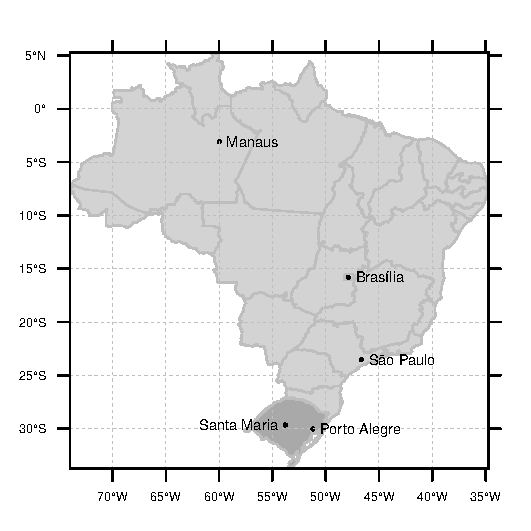
\includegraphics[width=90mm]{chap01FIG1a}
    \end{minipage}
    \begin{minipage}[b]{95mm}
      \subcaption{}
      \label{fig:points}
      \centering
      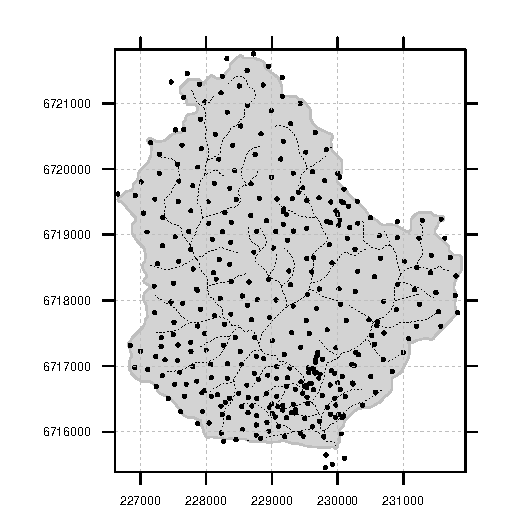
\includegraphics[width=90mm]{chap01FIG1b}
    \end{minipage}
  \caption{Location of the study area (a) in the central region of the 
  southernmost Brazilian state, Rio Grande do Sul, and the spatial distribution 
  of the $n=350$ point soil observations (b) made between the years of 2008 and
  2011 as part of soil and land use mapping projects.}
  \label{fig:location-intro}
\end{figure}

The soil database is composed by $n=350$ point observations. They were sampled 
during a soil and land use survey started in 2008 and published in the scale of
1:30,000 \cite{SamuelRosaEtAl2011a, MiguelEtAl2012}. Soil data includes 
particle size distribution, organic carbon content, bulk density, and effective 
cation exchange capacity. Environmental covariates include 20 data layers freely
available for the study area. They include information on relief, vegetation, 
land use, geology, soil parent material, soil (taxa) and intimately-associated 
surface conditions.

\subsection{Outline}

The thesis is composed of three core chapters. Each chapter deals with one specific 
research question and specific objective. Chapter 1 will deal with assessing 
whether investing in more accurate covariates improves prediction accuracy. 
Chapter 2 will deal with identifying appropriate calibration sample sizes and 
sampling designs for building DSM models for mapping soil properties. Chapter 3 
will deal with evaluating automated methods used to select covariates to build 
linear DSM models on how they affect model composition and prediction accuracy.
